\chapter{Experimental Results and Discussion}
\label{ch:results}
This chapter reports the experiments run on the prototype of Chapter~7 and discusses what they show. Every result in this chapter comes from simulated data in which a known share of facial variation was planted. The experiments therefore answer one kind of question, which is whether the pipeline and the models behave correctly, and they cannot answer the other kind, which is how well genotype predicts real faces. The chapter first states the experimental setup, then reports the validation of the pipeline, the comparison of models, the effect of sample size, the recovery of published associations, and the appearance integration. It then repeats the central experiments with real human genotypes in place of simulated ones, which removes the main simplifications of the generator while leaving the faces simulated. It closes with a discussion organised by research question and a statement of limitations.

\section{Experimental Setup}
The main experiments use the matched simulated cohort of Section~\ref{sec:impl-cohort}: 3{,}118 subjects, 5{,}000 SNPs, and a 50-dimensional shape target composed of 20 per cent genetic, 35 per cent demographic, and 45 per cent noise variance. The cohort is divided at subject level into 2{,}182 training, 467 validation, and 469 test subjects. All scaling, component fitting, and SNP screening use the training set only. Hyperparameters and stopping points are chosen on the validation set, and the test set is scored once.

The main measure is the coefficient of determination $R^2$ between predicted and true shape vectors, averaged over the 50 dimensions and computed on the test set. A value of zero corresponds to predicting the training mean face, and a value of one to perfect prediction. Mean error per vertex of the decoded mesh, in millimetres, is reported where it helps interpretation.

Two kinds of repetition are used and should not be confused. The linear analyses of Section~\ref{sec:res-controls} are repeated over five independently generated cohorts, with 95 per cent confidence intervals obtained by resampling test subjects. The neural models of Section~\ref{sec:res-models} are trained three times with different random initialisations on one cohort and one split, so the spread reported for them reflects initialisation only. Differences between neural models smaller than about 0.01 in $R^2$ should not be read as real. The neural experiments ran on an NVIDIA RTX A4000 graphics card and took about 49 minutes in total.

\section{Validation of the Pipeline}
\label{sec:res-controls}
Before comparing models, we tested whether the pipeline can detect genetic signal at all, and whether it stays silent when there is none. Table~\ref{tab:res-ladder} and Figure~\ref{fig:res-ladder} report a ladder of linear models, each given more information than the last.

\begin{table}[!ht]
\centering
\caption{Baseline ladder on the matched simulated cohort. Test $R^2$, mean and standard deviation over five generated cohorts.}
\label{tab:res-ladder}
\small
\begin{tabular}{|p{8.4cm}|p{2.6cm}|p{3.3cm}|}
\hline
\textbf{Model} & \textbf{Test $R^2$} & \textbf{Gain over row 3} \\ \hline
1. Mean face & $-0.002 \pm 0.000$ & --- \\ \hline
2. Covariates (sex, age, age squared, height, weight) & $0.205 \pm 0.015$ & --- \\ \hline
3. Covariates and ten ancestry principal components & $0.315 \pm 0.003$ & reference \\ \hline
4. Row 3 and 256 SNP principal components & $0.319 \pm 0.004$ & $+0.004$ \\ \hline
5. Row 3 and screened SNPs (ridge regression) & $0.488 \pm 0.004$ & $+0.173$ \\ \hline
6. Row 3 and the true causal SNPs (oracle) & $0.488 \pm 0.005$ & $+0.173$ \\ \hline
\end{tabular}
\end{table}

\begin{figure}[!ht]
\centering
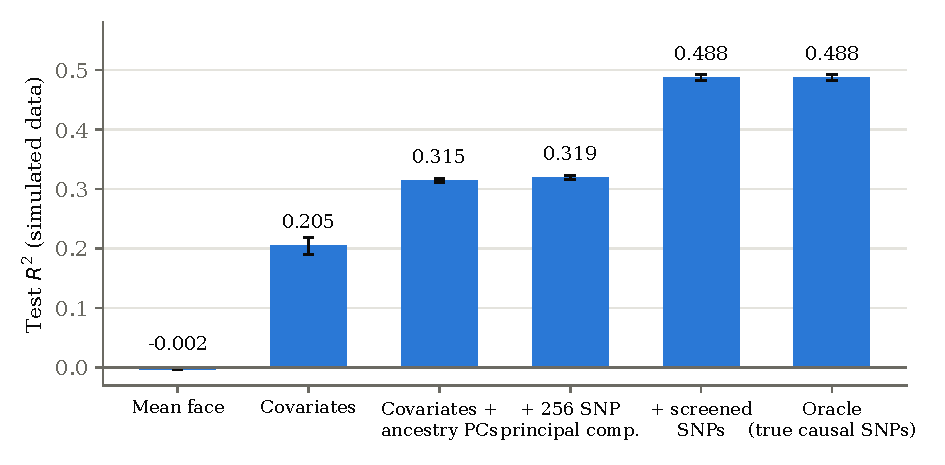
\includegraphics[width=0.86\textwidth]{Figures/res_ladder.pdf}
\caption{Baseline ladder on the matched simulated cohort. Error bars show the standard deviation over five generated cohorts.}
\label{fig:res-ladder}
\end{figure}

Three observations follow. First, ancestry components add 0.110 over the other covariates, which confirms that the simulated cohort contains the population structure it was designed to contain, and that a baseline without ancestry would flatter any genetic model. In the simulation, ten ancestry components estimated from genotype do as well as the true ancestry labels ($0.315$ against $0.316$), so the baseline does not depend on information that real data would lack.

Second, the oracle shows that SNPs can add $0.173$ beyond covariates and ancestry. A ridge regression on screened SNPs recovers all of it, with per-cohort confidence intervals lying between $+0.159$ and $+0.188$. The pipeline therefore finds the planted signal.

Third, the same SNPs passed through 256 principal components add only $0.004$. This matters because our first round of experiments used that representation alone, and on that basis we had provisionally concluded that SNPs added nothing beyond demographics. The oracle exposed that conclusion as an artefact of our own feature step. The leading components of unlinked SNPs capture ancestry, which the baseline already has, and discard the small individual effects that carry the planted signal. We report this openly, because the correction is the most useful methodological lesson of this phase: a null result is trustworthy only if a positive control shows that the method could have found an effect.

Table~\ref{tab:res-neg} reports the negative controls. When genotype rows are shuffled so that faces and genotypes no longer belong together, and when the cohort is regenerated with no genetic contribution, the gain from SNPs is $-0.001$ in both cases. The small negative value is expected, since fitting uninformative features costs a little accuracy. No confidence interval lies above zero. The pipeline therefore reports no signal where none exists, which rules out leakage between the training and test sets.

\begin{table}[!ht]
\centering
\caption{Positive and negative controls. Gain in test $R^2$ from adding screened SNPs to covariates and ancestry components.}
\label{tab:res-neg}
\small
\begin{tabular}{|p{8.6cm}|p{2.2cm}|p{3.5cm}|}
\hline
\textbf{Condition} & \textbf{Gain} & \textbf{Expected} \\ \hline
Planted genetic share of 0.20 (five cohorts) & $+0.173$ & clearly above zero \\ \hline
Genotype rows shuffled (five cohorts) & $-0.001$ & zero \\ \hline
Planted genetic share of zero (three cohorts) & $-0.001$ & zero \\ \hline
\end{tabular}
\end{table}

\section{Comparison of Models}
\label{sec:res-models}
With the pipeline validated, the four neural models were compared with the demographic baseline, each given the demographic covariates together with one of the two SNP representations of Section~\ref{sec:impl-features}. Table~\ref{tab:res-models} and Figure~\ref{fig:res-models} give the results.

\begin{table}[!ht]
\centering
\caption{Neural models on the matched simulated cohort. Test $R^2$, mean and standard deviation over three training runs. The demographic baseline scores $0.317$.}
\label{tab:res-models}
\small
\begin{tabular}{|p{4.6cm}|p{3.6cm}|p{3.1cm}|p{2.9cm}|}
\hline
\textbf{Model} & \textbf{256 SNP principal components} & \textbf{256 screened SNPs} & \textbf{Mesh error, screened (mm)} \\ \hline
Demographics only (baseline) & $0.317$ & $0.317$ & $3.00$ \\ \hline
Multilayer perceptron & $0.274 \pm 0.001$ & $0.396 \pm 0.002$ & $2.79$ \\ \hline
Contrastive model & $0.220 \pm 0.004$ & $0.364 \pm 0.001$ & $2.88$ \\ \hline
Transformer encoder & $0.311 \pm 0.005$ & $0.319 \pm 0.002$ & $3.00$ \\ \hline
Conditional diffusion & $-0.368 \pm 0.006$ & $0.081 \pm 0.006$ & $3.38$ \\ \hline
\end{tabular}
\end{table}

\begin{figure}[!ht]
\centering
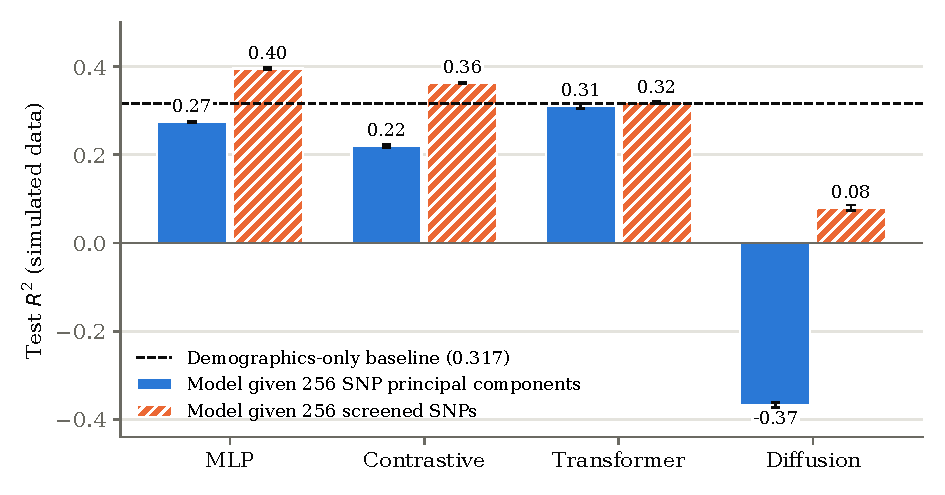
\includegraphics[width=0.86\textwidth]{Figures/res_models.pdf}
\caption{Neural models with two SNP representations, against the demographic baseline. Error bars show the standard deviation over three training runs.}
\label{fig:res-models}
\end{figure}

With principal components, no neural model exceeds the demographic baseline, which agrees with the finding of Section~\ref{sec:res-controls} that this representation carries almost no usable genetic signal. With screened SNPs, the multilayer perceptron and the contrastive model both exceed the baseline clearly, by $0.079$ and $0.047$. The mean mesh error of the multilayer perceptron falls from $3.00$ to $2.79$ millimetres. The Transformer stays at the baseline, and the diffusion model remains far below it, although it improves greatly over its result with principal components.

The choice of SNP representation therefore mattered more than the choice of architecture. The same multilayer perceptron moves from below the baseline to well above it when only its input changes.

The comparison with the linear reference is the central result for the question of model complexity. The best neural model recovers $0.079$ of the $0.173$ that is available, less than half, while the tuned ridge regression of Table~\ref{tab:res-ladder} recovers all of it. The two figures come from different scripts, and the ridge regression was tuned over the number of SNPs while the neural models were given a fixed 256, so the comparison is indicative and not exact. The gap of about $0.09$ is nevertheless far larger than any difference that this could explain. This result must be read with the design of the simulation in mind. The planted effects are linear and additive, so a linear model is the correctly specified one. The experiment shows that the neural models are less efficient at learning a linear signal from about two thousand subjects. It does not show that neural models are worse in general, and it cannot show whether real facial genetics contains non-linear structure that would favour them.

The shuffled-genotype control was also applied to the neural models, with one training run each. The Transformer scored $0.316$, the multilayer perceptron $0.252$, and the contrastive model $0.247$, against $0.317$ for the baseline. No model gains from uninformative SNPs, which again rules out leakage. Two further points follow. The multilayer perceptron and the contrastive model lose about $0.07$ when given uninformative SNPs, so on data with very weak genetic signal they could fall below the demographic baseline. The Transformer scores the same with shuffled and with real genotypes, which indicates that at this sample size it is not using the SNPs at all.

\section{Effect of Sample Size}
To ask whether more subjects would change these conclusions, a separate cohort of 10{,}000 subjects was generated with the same settings. Models were trained on nested subsets of its training set and scored on one fixed test set of 1{,}500 subjects. This is a scaling experiment only. The real cohort has 3{,}118 subjects, so results beyond the first row of Table~\ref{tab:res-scaling} describe a cohort that we will not have.

\begin{table}[!ht]
\centering
\caption{Effect of training-set size, with screened SNPs. Test $R^2$, mean over three training runs. Standard deviations are at most $0.003$ except for the diffusion model, where they reach $0.012$.}
\label{tab:res-scaling}
\small
\begin{tabular}{|p{2.5cm}|p{2.4cm}|p{2.0cm}|p{2.2cm}|p{2.3cm}|p{1.9cm}|}
\hline
\textbf{Training subjects} & \textbf{Demographics} & \textbf{Multilayer perceptron} & \textbf{Contrastive} & \textbf{Transformer} & \textbf{Diffusion} \\ \hline
2{,}182 & $0.312$ & $0.389$ & $0.349$ & $0.310$ & $0.058$ \\ \hline
4{,}000 & $0.313$ & $0.417$ & $0.392$ & $0.316$ & $0.049$ \\ \hline
7{,}000 & $0.314$ & $0.435$ & $0.428$ & $0.338$ & $0.028$ \\ \hline
\end{tabular}
\end{table}

\begin{figure}[!ht]
\centering
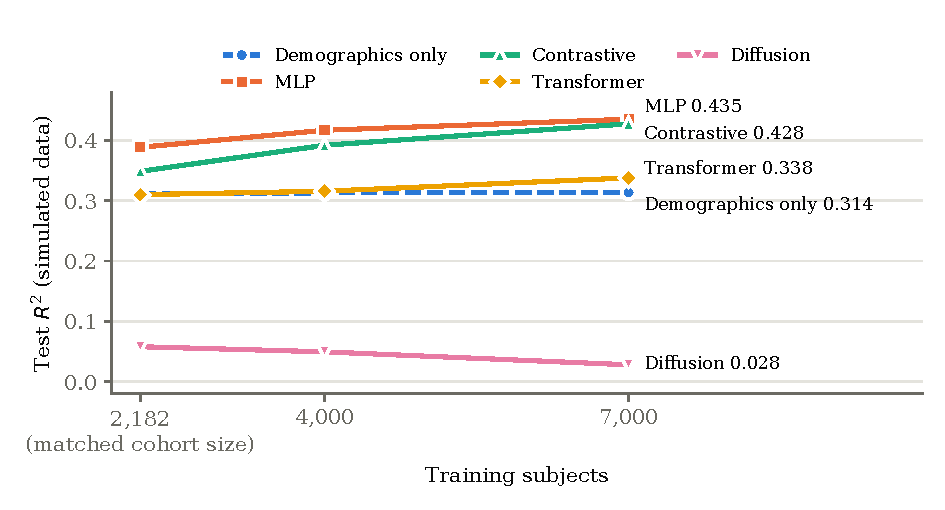
\includegraphics[width=0.86\textwidth]{Figures/res_scaling.pdf}
\caption{Effect of training-set size on each model, with screened SNPs.}
\label{fig:res-scaling}
\end{figure}

The demographic baseline is flat, as expected for a linear model with a handful of inputs. The multilayer perceptron gains $0.046$ and the contrastive model $0.079$ from roughly three times the data, and the contrastive model nearly closes its gap to the multilayer perceptron. The Transformer begins to exceed the baseline only at 7{,}000 subjects. The diffusion model does not improve with more data. We have not diagnosed the cause, and we report it as an open negative result.

Table~\ref{tab:res-power} gives a companion analysis with the linear screen, over cohort sizes and planted genetic shares. At the size of the real cohort, SNPs add $0.070$ when the planted share is 0.10 and $0.177$ when it is 0.20, and nothing when it is zero. These figures are an optimistic upper bound and not a forecast for real data, for the reasons given in Section~\ref{sec:res-limits}.

\begin{table}[!ht]
\centering
\caption{Gain in test $R^2$ from screened SNPs, by cohort size and planted genetic share. Mean of two generated cohorts.}
\label{tab:res-power}
\small
\begin{tabular}{|p{3.2cm}|p{3.0cm}|p{3.0cm}|p{3.0cm}|}
\hline
\textbf{Cohort size} & \textbf{Share 0.00} & \textbf{Share 0.10} & \textbf{Share 0.20} \\ \hline
1{,}000 & $-0.000$ & $+0.022$ & $+0.119$ \\ \hline
2{,}000 & $-0.001$ & $+0.055$ & $+0.157$ \\ \hline
3{,}118 & $-0.001$ & $+0.070$ & $+0.177$ \\ \hline
6{,}000 & $-0.001$ & $+0.087$ & $+0.192$ \\ \hline
\end{tabular}
\end{table}

\section{Recovery of Published Associations}
Section~\ref{sec:impl-inject} described how 14 published associations between lead SNPs and facial measurements were added to the simulated measurements. To check that the evaluation can recover known associations and only those, every one of the 260 pairs of SNP and measurement was tested after adjusting both for sex, age, age squared, height, weight, and ancestry. All 14 injected pairs were detected at a Bonferroni threshold, each with the published direction of effect. None of the 246 pairs that were not injected was detected, and 2.8 per cent of them fell below 0.05, which is consistent with chance. On the larger cohort of 10{,}000 subjects the result was the same, with 6.1 per cent of the remaining pairs below 0.05.

This result confirms that the association machinery is correct and that adjustment for ancestry prevents false associations in a structured cohort. It is not a replication of the published associations. The signals were placed in the data by us, so finding them shows that the method works and nothing more.

\section{Appearance Integration}
\label{sec:res-app-sim}
The appearance module was applied to the 41 marker SNPs of every subject in the matched simulated cohort. Table~\ref{tab:res-app} gives the distribution of the predicted categories.

\begin{table}[!ht]
\centering
\caption{Predicted appearance categories on the matched simulated cohort, as a percentage of subjects. These describe the simulation only.}
\label{tab:res-app}
\small
\begin{tabular}{|p{2.6cm}|p{11.6cm}|}
\hline
\textbf{Trait} & \textbf{Predicted categories} \\ \hline
Eye colour & blue 54.7, brown 44.1, intermediate 1.2 \\ \hline
Hair colour & brown 68.8, blond 17.9, red 8.6, black 4.7 \\ \hline
Hair shade & light 63.0, dark 37.0 \\ \hline
Skin colour & intermediate 72.5, pale 14.0, very pale 12.2, dark to black 1.1, dark 0.3 \\ \hline
\end{tabular}
\end{table}

These figures show that the module runs end to end on the same genotype file as the shape models and returns a varied and plausible mix of categories, which is what RQ8 asks of the integration. They are not a measure of accuracy. The marker frequencies in the simulation are synthetic and the cohort has no colour labels to compare against.

\subsection{Why the Colour Component Was Not Tested on Real People}
\label{sec:res-appearance-untested}
Colour is the one part of FaceCon that could in principle have been checked against real human phenotypes, because the model is a published one that this project did not fit, and because self-reported eye colour is the kind of label an open cohort might carry. The check was written: it maps survey answers onto the model's three categories, scores one-against-rest areas under the curve, and compares them against a null built from a thousand label shuffles. It was validated end to end on a stand-in cohort, where it proved sensitive to the direction of the labels, scoring $0.995$ with them correctly oriented and $0.000$ reversed, with the shuffled null centred on one half as it should be.

It was never run, because the data source stopped serving. The intended cohort was the Harvard Personal Genome Project, whose participants publish genotype files and trait surveys under a public-domain dedication, making it usable without an access application. Its site now answers every request with a redirect to the identical address, over both plain and encrypted connections and regardless of the client, which no client can resolve; a separate fault leaves its certificate valid only for a hostname that forwards to the one that loops. The other candidate, openSNP, which paired consumer genotypes with self-reported traits, shut down permanently in April 2025 and deleted its data.

This is worth stating as more than an inconvenience. The open genotype-and-phenotype resources on which an independent check of a published appearance model depends have largely ceased to exist, and a project without institutional data access has no remaining route to one. FaceCon therefore reports its colour component as integrated and faithful to the official calculator, and makes no claim whatever about its accuracy on real people. That silence is not a choice of scope: it is the honest consequence of there being nothing left to test against.

\section{Experiments on Real Genotypes}
\label{sec:res-real}
The experiments reported so far use genotypes that we generated ourselves, and Section~\ref{sec:res-limits} identifies three ways in which such genotypes are easier than real ones. They are statistically independent of one another, whereas real SNPs that sit close together on a chromosome are correlated. Their allele frequencies are drawn from a convenient range. Their ancestry groups are cleanly separated, whereas real population structure is continuous. To remove these three advantages, the experiment was repeated with real human genotypes in place of simulated ones, using the panel described in Section~\ref{sec:impl-1kg}. The faces remain simulated, so this experiment is still not a statement about real faces. What changes is that the genotype side of the problem is now real.

The cohort holds 2{,}573 unrelated people from the 1000 Genomes Project and 100{,}009 SNPs, divided into 1{,}801 training, 385 validation, and 387 test subjects. The five continental groups are unevenly represented, with 680 African, 525 European, 511 South Asian, 506 East Asian, and 351 American subjects, which is itself more realistic than the balanced groups of the simulation. The planted genetic share is again 0.20, but the effects are now sparse, with 300 causal SNPs each affecting 5 of the 50 shape dimensions rather than all of them. Table~\ref{tab:res-kg-ladder} gives the baseline ladder, and the left panel of Figure~\ref{fig:res-kg} shows what SNPs add.

\begin{table}[!ht]
\centering
\caption{Baseline ladder on real genotypes with simulated faces. Test $R^2$, mean and standard deviation over five generated cohorts.}
\label{tab:res-kg-ladder}
\small
\begin{tabular}{|p{8.4cm}|p{2.6cm}|p{3.3cm}|}
\hline
\textbf{Model} & \textbf{Test $R^2$} & \textbf{Gain over row 3} \\ \hline
1. Mean face & $-0.003 \pm 0.000$ & --- \\ \hline
2. Covariates (sex, age, age squared, height, weight) & $0.195 \pm 0.010$ & --- \\ \hline
3. Covariates and ten ancestry principal components & $0.335 \pm 0.008$ & reference \\ \hline
4. Row 3 and 256 SNP principal components & $0.335 \pm 0.009$ & $+0.001$ \\ \hline
5. Row 3 and screened SNPs (ridge regression) & $0.435 \pm 0.006$ & $+0.100$ \\ \hline
6. Row 3 and the true causal SNPs (oracle) & $0.449 \pm 0.005$ & $+0.114$ \\ \hline
\end{tabular}
\end{table}

The pattern of Section~\ref{sec:res-controls} survives the change of genotypes, with two differences worth recording. The oracle now adds $0.114$ and the screen recovers $0.100$ of it, which is 88 per cent rather than all of it. Real correlation between SNPs makes the causal ones harder to isolate, which is the expected direction. The 256 principal components add $0.001$, which is zero to the precision that matters, so the finding that this representation discards the genetic signal is not an artefact of unlinked simulated SNPs. A second difference appears one row higher. True ancestry labels score $0.345$ against $0.335$ for ten estimated components, a gap that was absent in the simulation, which is what continuous population structure should do to a fixed number of components.

\begin{figure}[!ht]
\centering
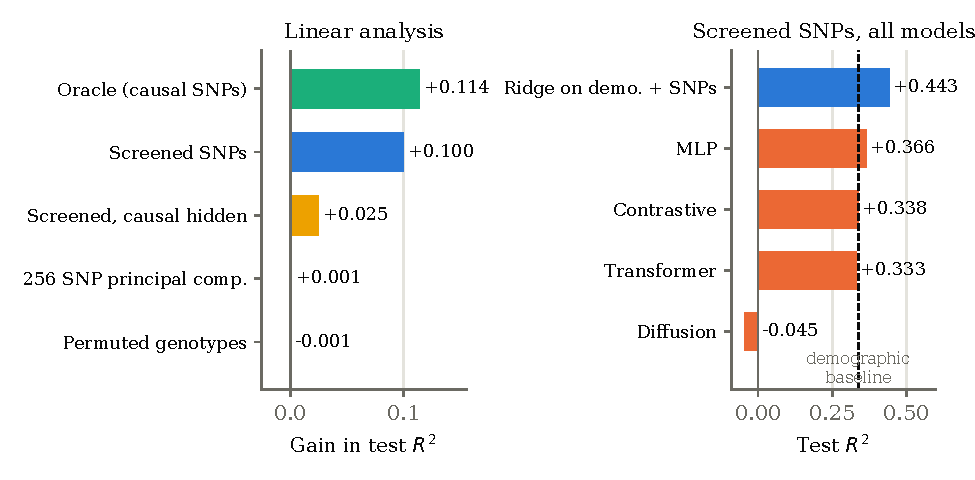
\includegraphics[width=0.92\textwidth]{Figures/res_kg.pdf}
\caption{Real genotypes with simulated faces. The left panel shows what SNPs add beyond covariates and ancestry components. The right panel compares the models with the linear reference on the same split.}
\label{fig:res-kg}
\end{figure}

\subsection{What Correlation Between SNPs Carries}
\label{sec:res-ld}
Real genotypes make a question possible that the simulation could not pose. In a real study the causal variant is usually not on the array, and an association is detected only because a nearby SNP is correlated with it. To measure how much of the signal survives that indirection, the analysis was repeated with the 300 causal SNPs deleted from the panel, so that no model could use them and only their neighbours remained.

Under this condition the screen adds $0.025$, against $0.114$ when the causal SNPs are available. Correlation between neighbouring SNPs therefore carries about 22 per cent of the available signal. The per-cohort confidence intervals lie between $+0.018$ and $+0.035$ and none includes zero, so the effect is real rather than noise. The same experiment on the simulated panel of Section~\ref{sec:res-controls} gives $-0.001$, as it must, because unlinked SNPs have no neighbours to carry anything. This is the clearest illustration in this report of why the realism of the genotype matters, and it offers a mechanism for an observation that is common in the published literature, namely that individual associated SNPs explain very little variance. A panel of common SNPs reads neighbours and not causes, and a fifth of the attainable signal is what that indirection leaves.

\subsection{Models Against the Linear Reference}
Table~\ref{tab:res-kg-models} compares the four neural models with two linear references on the same cohort and the same split. The first reference uses the demographic covariates alone. The second is given exactly what the neural models are given, which is the covariates together with the SNP features, and is fitted in two stages so that the covariates are not penalised. This second reference did not exist for the experiments of Section~\ref{sec:res-models}, where the linear and neural results came from different scripts and could only be compared indirectly. Here the comparison is exact.

\begin{table}[!ht]
\centering
\caption{Models on real genotypes with simulated faces. Test $R^2$, mean and standard deviation over three training runs. The linear references are fitted once and have no spread, and the permuted column is a single run of each model.}
\label{tab:res-kg-models}
\small
\begin{tabular}{|p{5.4cm}|p{3.4cm}|p{3.0cm}|p{2.2cm}|}
\hline
\textbf{Model} & \textbf{256 SNP principal components} & \textbf{256 screened SNPs} & \textbf{Permuted genotypes} \\ \hline
Demographics only (baseline) & $0.338$ & $0.338$ & $0.338$ \\ \hline
Ridge on demographics and SNPs & $0.338$ & $0.443$ & $0.338$ \\ \hline
Multilayer perceptron & $0.242 \pm 0.002$ & $0.366 \pm 0.001$ & $0.243$ \\ \hline
Transformer encoder & $0.327 \pm 0.001$ & $0.333 \pm 0.001$ & $0.330$ \\ \hline
Contrastive model & $0.175 \pm 0.002$ & $0.338 \pm 0.002$ & $0.239$ \\ \hline
Conditional diffusion & $-0.523 \pm 0.034$ & $-0.045 \pm 0.014$ & $-0.291$ \\ \hline
\end{tabular}
\end{table}

The linear reference adds $0.106$ over the demographic baseline. The baseline ladder of Table~\ref{tab:res-kg-ladder} measures a closely related quantity with separate fitting and scoring code, ten ancestry components in place of ancestry labels, and a number of SNPs tuned on the validation set rather than a fixed 256. The first of its five cohorts is the cohort used here, with the same subjects and the same split, and on it the controls script reports a gain of $0.105$. Two implementations that differ in all of these respects agreeing to within $0.001$ on the same subjects is the strongest evidence available to us that neither contains an error in the direction that matters. Averaged over all five cohorts, the gain is $0.100$.

The best neural model adds $0.028$, which is a quarter of what the linear reference adds and a quarter of what the oracle makes available. The gap between the best neural model and the linear reference is $0.077$ on the same split. Only the multilayer perceptron responds to the genotypes at all. The Transformer scores $0.333$ with real SNPs and $0.330$ with permuted ones, a difference within its run-to-run spread, so it is reading the covariates and ignoring the genotypes. The contrastive model lands exactly on the demographic baseline. The diffusion model remains below the mean face and is worse here than on the simulated panel.

With principal components, every neural model falls at or below the demographic baseline, and the linear reference given the same features scores exactly the baseline value. When a correctly specified linear model extracts nothing from a representation, the representation contains nothing to extract, and the failure of the neural models on these features cannot be attributed to the models.

\subsection{Controls on the Real Panel}
Both negative controls were repeated. With genotype rows shuffled, the linear reference scores $0.338$, which is the demographic baseline to three decimal places, and every neural model scores at or below it. The acceptance check that no model gains more than $0.01$ over the baseline passes for the neural models and for the linear reference.

The second of these checks was added after an error of our own. The linear reference was first written as a single ridge regression over the covariates and the SNP features together, which penalises the covariates alongside the SNPs. On permuted genotypes that version scored $0.207$ against a baseline of $0.317$, because the large penalty that uninformative features require also shrinks the covariates that carry real information. It would have understated the linear option precisely where the comparison with the neural models is strictest. The two-stage form used in Table~\ref{tab:res-kg-models} fits the covariates without penalty and then fits the SNP features to what the covariates leave over, and returns the baseline value exactly under permutation. The check is now part of the suite so that the error cannot return unnoticed.

The association analysis of Section~\ref{sec:impl-inject} was also repeated on the real panel. All 14 injected associations were recovered with the published direction, no Bonferroni detection appeared among the 246 pairs that were not injected, and 6.1 per cent of them fell below 0.05. Real correlation between SNPs did not create false associations once ancestry was adjusted for.

The frequency check described in Section~\ref{sec:impl-1kg} flagged 2 of the 13 published lead SNPs, whose frequency in the European subjects of the panel differs from the published one by more than the tolerance. Both are insertions or deletions, for which the identifier in the 1000 Genomes files refers to a different representation of the variant than the published table does. Neither reached genome-wide significance in the source study, and both carry weights that we planted rather than published ones, so no result in this chapter depends on their alignment. They are reported because the check exists in order to be acted on rather than passed over.

\subsection{Appearance on Real Genotypes}
The appearance module was applied to the real marker genotypes of the same people. Of the 41 markers, 39 are present in the panel. The two that are absent, N29insA and Y152OCH, are rare variants of the MC1R gene associated with red hair, and treating every subject as a non-carrier of them will understate red hair. Table~\ref{tab:res-kg-app} gives the most frequent predicted category for each trait and group.

\begin{table}[!ht]
\centering
\caption{Most frequent predicted appearance category by continental group, on real marker genotypes, as a percentage of subjects in the group. These are plausibility checks and not measures of accuracy.}
\label{tab:res-kg-app}
\small
\begin{tabular}{|p{2.9cm}|p{3.7cm}|p{3.5cm}|p{3.9cm}|}
\hline
\textbf{Group} & \textbf{Eye colour} & \textbf{Hair colour} & \textbf{Skin colour} \\ \hline
African & brown 99.7 & black 94.1 & dark to black 99.1 \\ \hline
East Asian & brown 100.0 & black 100.0 & dark to black 89.5 \\ \hline
South Asian & brown 99.8 & black 82.0 & dark to black 52.6 \\ \hline
American & brown 94.3 & black 49.6 & dark to black 40.5 \\ \hline
European & brown 52.0 & brown 57.1 & intermediate 89.9 \\ \hline
\end{tabular}
\end{table}

The predictions vary between groups in the direction that the published model predicts, with blue eyes and lighter skin far more frequent among Europeans than among the other groups. This is a stronger check than the one in Section~\ref{sec:res-app-sim}, because the marker genotypes are real rather than simulated. It remains a plausibility check and not an accuracy measurement, since the 1000 Genomes Project records no eye, hair, or skin colour for its subjects, so there is nothing to compare the predictions against.

\subsection{What This Experiment Does and Does Not Establish}
Three of the advantages that the simulation gave the method have been removed, and the main conclusions survive. SNPs add a measurable amount beyond covariates and ancestry, principal components discard that signal, the pipeline stays silent under permutation, and a regularised linear model beats every neural model. Two new results appear, namely that correlation between SNPs carries about a fifth of the attainable signal, and that the gap between neural and linear models is $0.077$ when both are given identical inputs on one split.

The limits of the experiment should be equally clear. The faces, ages, heights, and weights are still simulated, and the mapping from genotype to face is one we imposed. That mapping is additive and linear, so the linear reference is the correctly specified model and is expected to win. The result shows that these neural models are inefficient at learning an additive signal from 1{,}801 training subjects, and it cannot show how they would behave on a signal with the non-linear structure that real facial genetics may or may not contain. The planted share of 0.20 is a design choice and not an estimate of the real one. For these reasons the figures in this section remain properties of the pipeline rather than facts about human faces.

\section{When the Signal Is Not Additive}
\label{sec:res-nonadd}
Every experiment reported so far planted an additive signal, in which each copy of an allele shifts the face by the same amount and no SNP depends on another. Section~\ref{sec:res-limits} lists that as a limitation: the linear reference is the correctly specified model for such a signal, so its victory over the neural models says nothing about a signal with structure. Real facial genetics may contain dominance, where the heterozygote does not sit midway between the two homozygotes, and epistasis, where the effect of one SNP depends on the genotype at another. Neither can be measured from data the project does not have. What can be done is to plant them deliberately and ask what the evaluation sees.

Four further cohorts were generated, identical to the matched cohort in every other respect, differing only in how the planted genetic share of 0.20 is divided. In the dominance cohort half of that share is carried by heterozygote deviations; in the epistasis cohort half is carried by products of pairs of centred genotypes; in the mixed cohort a third goes to each. The additive cohort is the original. Two rows were added to the ladder for these cohorts. The first, written \mbox{+SNP-screen-NA}, replaces the single additive screen with a two-degree-of-freedom score that tests each SNP's additive and heterozygote terms together and keeps both columns for the SNPs it selects. The second, ORACLE-NA, is given the true causal SNPs, the true heterozygote codes, and the true interacting pairs. Table~\ref{tab:res-nonadd} reports the gain of each row over the \mbox{cov+PC} baseline, averaged over the same five cohorts used throughout.

\begin{table}[!ht]
\centering
\caption{Gain in $R^2$ over the covariates-and-components baseline when the planted signal is not additive. Five cohorts per arm. The calibration arm is the same additive cohort with the two extra rows also fitted, which is what makes the cost of those rows visible. All faces are simulated and the architecture is one we imposed.}
\label{tab:res-nonadd}
\small\setstretch{1.15}
\begin{tabular}{|p{3.3cm}|p{2.0cm}|p{2.0cm}|p{2.0cm}|p{2.0cm}|p{1.9cm}|}
\hline
\textbf{Row} & \textbf{Additive} & \textbf{Calibration} & \textbf{Dominance} & \textbf{Epistasis} & \textbf{Mixed} \\ \hline
+SNP-screen    & $+0.1726$ & $+0.1726$ & $+0.0987$ & $+0.0699$ & $+0.0565$ \\ \hline
+SNP-screen-NA & ---       & $+0.1501$ & $+0.1536$ & $+0.0523$ & $+0.0884$ \\ \hline
ORACLE         & $+0.1729$ & $+0.1729$ & $+0.0987$ & $+0.0717$ & $+0.0581$ \\ \hline
ORACLE-NA      & ---       & $+0.1429$ & $+0.1451$ & $+0.1475$ & $+0.1477$ \\ \hline
Permuted genotypes & $-0.0006$ & $-0.0006$ & $-0.0007$ & $-0.0007$ & $-0.0007$ \\ \hline
Zero genetic share & $-0.0011$ & $-0.0011$ & $-0.0011$ & $-0.0011$ & $-0.0011$ \\ \hline
\end{tabular}
\end{table}

\begin{figure}[!ht]
\centering
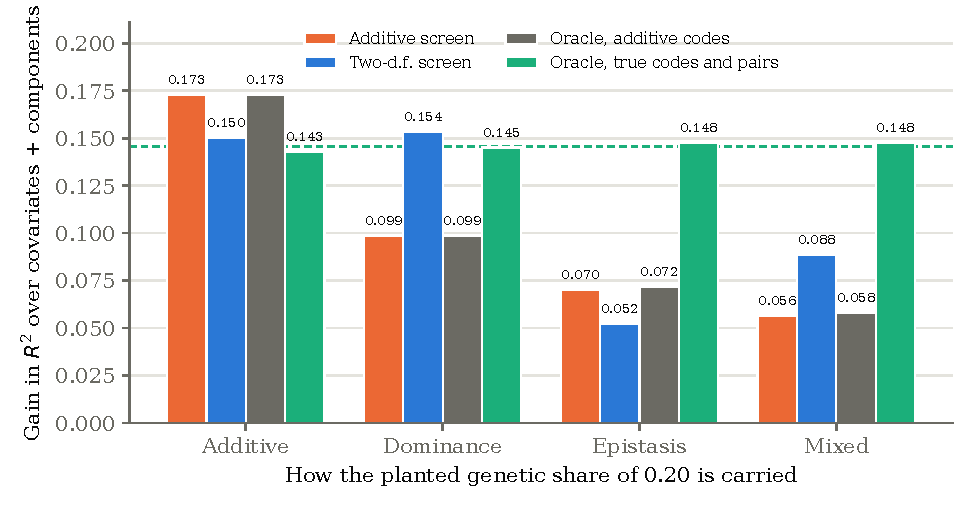
\includegraphics[width=\textwidth]{Figures/res_nonadd.pdf}
\caption{What each model recovers as the form of the planted signal changes, while its total size stays at 0.20. The dashed line marks the mean of the oracle given the true codes and pairs, which is nearly flat across all four architectures; the additive models fall away from it. Simulated faces, imposed architecture.}
\label{fig:res-nonadd}
\end{figure}

The last two rows come first, because without them the rest would not be interpretable. Permuting the genotypes and setting the genetic share to zero both return approximately zero in every arm, so the extra rows have not introduced a way of finding signal that is not there.

The main result, drawn in Figure~\ref{fig:res-nonadd}, is in the ORACLE-NA row. Given the right representation, the recoverable signal is almost the same in all four arms, between $0.143$ and $0.148$, which is what should happen: the same total share of 0.20 was planted each time and only its form was changed. The additive oracle, by contrast, falls from $0.173$ on the additive cohort to $0.058$ on the mixed one. A model restricted to additive allele dosages therefore sees about a third of a signal that is in fact fully present in the genotypes. This is the clearest statement this project can make about why published association studies report small individual effects: part of the shortfall need not be absent signal at all, but signal in a form that the standard additive model cannot express.

The practical rows behave less tidily, and in one case worse than the additive row they were meant to improve on. On the dominance cohort the two-degree-of-freedom screen gains $0.1536$ against the additive screen's $0.0987$, and on the mixed cohort $0.0884$ against $0.0565$. On the epistasis cohort it gains $0.0523$ against $0.0699$, which is to say it is worse than doing nothing. This was not expected, and Section~\ref{sec:res-nonadd-honest} sets out why it happens and what was and was not done about it.

\subsection{Two Expectations That Were Wrong}
\label{sec:res-nonadd-honest}
This experiment was pre-registered before any of its numbers were read, with the thresholds and the expected direction of each row written down in advance. Two of those expectations turned out to be wrong, and both are recorded here rather than quietly corrected, because a protocol that is only reported when it agrees with the result is not a protocol.

The first concerns the cost of the extra rows. Fitting dominance and interaction columns on a cohort where they carry nothing cannot help, and was expected to cost about $0.02$ in $R^2$. The measured cost is larger: ORACLE sits $0.030$ above ORACLE-NA on the additive-calibration arm averaged over five cohorts, and $0.032$ on a single cohort. The pre-registered figure was not loosened to accommodate this. The consequence matters for reading Table~\ref{tab:res-nonadd}: ORACLE-NA is not a drop-in replacement for ORACLE, the two are comparable only within an arm, and the fact that ORACLE-NA is the lower of the two on the additive cohort is the expected direction and not a failure. Because the cost is of the same order as some of the gains in the table, it has to be stated plainly; a reader comparing ORACLE-NA on the mixed cohort against ORACLE on the additive one would otherwise read a modelling cost as a loss of signal.

The second concerns the epistasis cohort. The screen was expected to beat the additive screen wherever the signal was not additive, and it does not. The reason is a property of the screen and not a fault in the data: its per-SNP score tests a genotype's own heterozygote deviation, so it has power against dominance and none against a product of two SNPs whose individual effects average out. On that cohort the extra column per SNP is noise, and it costs what the paragraph above measures. The pre-registered expectation was wrong to treat non-additive as a single case. That the signal is nonetheless there is settled by ORACLE-NA, which recovers $0.1475$ on the same cohort when it is told which pairs interact; what fails is finding the pairs, not representing them.

No pair-aware screen was added in response. Designing a method after seeing which cohort defeated the existing one, and then reporting its success on that same cohort, would produce a number that means nothing. A screen over candidate pairs is named as future work in Chapter~\ref{ch:conclusion}, to be specified before it is run.

\subsection{The Neural Models on Non-Additive Signal}
\label{sec:res-nonadd-neural}
Chapter~\ref{ch:results} has so far reported that the regularised linear model beats every neural model, with the caveat that the planted signal was additive and the linear model was therefore correctly specified. The cohorts of Section~\ref{sec:res-nonadd} remove that caveat: a third of the genetic share is carried by heterozygote deviations and a third by interactions between pairs, so the linear model on additive dosages is now the wrong model, and the comparison is one the neural models should be expected to win. The pre-registered primary comparison is the best neural model minus the ridge on demographics and SNPs, on the two-degree-of-freedom features, paired within each of three independently generated cohorts.

\begin{table}[!ht]
\centering
\caption{Test parameter $R^2$ on the mixed-architecture cohorts, mean and standard deviation over three independently generated cohorts. The gap is the best neural model minus the ridge, paired within cohort, with a $t$ interval over the three.}
\label{tab:res-nonadd-neural}
\small\setstretch{1.15}
\begin{tabular}{|p{3.1cm}|p{2.3cm}|p{2.3cm}|p{2.0cm}|p{2.2cm}|p{2.6cm}|}
\hline
\textbf{Features} & \textbf{Demographics} & \textbf{Ridge, demo.\ + SNP} & \textbf{MLP} & \textbf{Transformer} & \textbf{Gap, best neural $-$ ridge} \\ \hline
Additive screen & $+0.307$ & $+0.344$ & $+0.294$ & $+0.306$ & $-0.038$ $[-0.050,-0.027]$ \\ \hline
Two-d.f.\ screen & $+0.307$ & $+0.391$ & $+0.326$ & $+0.306$ & $-0.065$ $[-0.070,-0.061]$ \\ \hline
Permuted control & $+0.308$ & $+0.308$ & $+0.251$ & $+0.304$ & --- \\ \hline
\end{tabular}
\end{table}

The ridge wins, and it wins by more than it did on additive signal. The gap is $-0.065$ with an interval that excludes zero comfortably, and it is wider on the two-degree-of-freedom features than on the additive ones. Removing the linear model's home advantage did not close the gap; it widened it. All four permuted negative controls pass, so none of this is an artefact of the models finding structure that is not there.

What separates the models is what each does with the better representation. Given the two-degree-of-freedom features in place of additive dosages, the ridge gains $0.047$, the MLP gains $0.032$, and the transformer gains nothing at all. The transformer is in fact the more striking case: at $+0.306$ it sits a thousandth below the demographics-only baseline on both feature sets, and it scores the same when the genotypes are permuted as when they are real. On this data, at this sample size, it is extracting no usable information from the genotypes whatsoever, and its apparent competence is entirely the covariates. The MLP does use the SNPs, since permuting them costs it $0.075$, but on additive features it still finishes $0.013$ below a model given only demographics, which is to say the SNP information it extracts does not pay for the overfitting it incurs.

The honest conclusion is narrow and should not be stretched. These two architectures, at this sample size, on these cohorts, cannot exploit non-additive structure that a linear model recovers from the same features. That is a statement about $n \approx 2{,}200$ training subjects and two specific architectures, not about neural networks and genetics in general; the published results that motivate such models use cohorts one to two orders of magnitude larger. What this project can say is that scale, not architecture, is the first thing to change, and that on a cohort of the size FaceCon expects, the representation handed to a regularised linear model matters more than the choice of network.

\section{Where the Gain Falls, and on Whom}
\label{sec:res-regional}
The results so far report one number for the whole face. Two questions ask for more detail. RQ6 asks whether some parts of the face are predicted better than others, and RQ7 asks whether the prediction works equally well for every ancestry group. Both were run on the real-genotype cohort, comparing the ridge model on covariates and screened SNPs against the demographic baseline, with confidence intervals from 2{,}000 bootstrap resamples of the test subjects.

\begin{table}[!ht]
\centering
\caption{Reduction in mean vertex error, in millimetres, from adding SNPs to the demographic baseline, by facial region and by ancestry group. Positive means the SNP model is closer to the simulated truth. Relative is the reduction as a percentage of the baseline error for that region.}
\label{tab:res-regional}
\small\setstretch{1.15}
\begin{tabular}{|p{3.4cm}|p{2.6cm}|p{2.4cm}|p{5.2cm}|}
\hline
\textbf{Region or group} & \textbf{Gain (mm)} & \textbf{Relative} & \textbf{Note} \\ \hline
Whole head & $0.356$ & $13.5$ per cent & 95 per cent interval $0.305$ to $0.408$ \\ \hline
Jaw & $0.567$ & $14$ per cent & largest absolute gain \\ \hline
Cheeks & $0.485$ & $14$ per cent & \\ \hline
Forehead & $0.337$ & $14$ per cent & \\ \hline
Mouth & $0.304$ & $14$ per cent & \\ \hline
Nose & $0.213$ & $13$ per cent & \\ \hline
Eyes & $0.203$ & $13$ per cent & smallest absolute gain \\ \hline
African group & $0.332$ & --- & intervals overlap \\ \hline
European group & $0.388$ & --- & intervals overlap \\ \hline
Other groups & $0.347$ & --- & intervals overlap \\ \hline
\end{tabular}
\end{table}

The absolute gains differ by a factor of nearly three between the jaw and the eyes, and it would be easy to present that as a finding about facial genetics. It is not one. In relative terms the gains are flat, between 13 and 14 per cent of the baseline error in every region, and the ordering of the absolute gains is simply the ordering of how much the regions vary in the first place. That is exactly what a signal planted uniformly across all 50 shape dimensions should produce, and it is what was planted. The honest reading is that this analysis confirms the regional measurement works and shows no region to be preferentially predictable. A real regional difference, if one exists, is not something this cohort can contain.

Two finer checks point the same way. Every one of the 68 landmarks improves, and so does every one of the 50 shape dimensions, with no dimension made worse by adding SNPs. A planted global effect predicts precisely that, and a real signal concentrated in a few features would not.

The same analysis on the 1000 Genomes cohort, where the genotypes are real and correlated, gives a smaller overall gain of $0.231$ mm $[0.188, 0.271]$ and the same flat profile: between $6.7$ and $8.6$ per cent of the baseline error across the six regions, against $13$ to $14$ per cent on the simulated panel. The ordering of the regions is nearly unchanged, with the forehead and mouth swapping places, which is the kind of movement a difference of this size should produce by chance. Again all 68 landmarks and all 50 dimensions improve. The MLP, run on the same cohort for comparison, gains $0.046$ mm with an interval of $[-0.008, 0.100]$ that includes zero, and improves only 54 of 68 landmarks and 34 of 50 dimensions, which is consistent with Section~\ref{sec:res-nonadd-neural}.

\subsection{What the Subgroup Result Does and Does Not Establish}
\label{sec:res-fairness}
On the 1000 Genomes cohort the five continental groups gain $0.186$ mm (AFR, $n=108$), $0.223$ (AMR, $n=55$), $0.268$ (EAS, $n=80$), $0.237$ (EUR, $n=68$) and $0.257$ (SAS, $n=76$). All five confidence intervals share the common range $[0.194, 0.260]$, so no difference between any pair can be claimed from this data.

That sentence is easy to misread, and the misreading matters more here than anywhere else in this report. Overlapping intervals at these sample sizes are not evidence that the groups are predicted equally well. The groups number between 55 and 108 test subjects, the intervals are correspondingly wide, and a real difference of the size seen in the point estimates would not be detected reliably at this $n$. The lowest point estimate is the African group's, which is $0.082$ mm or about a third below the highest, and that is the direction a reader should be most alert to: African-ancestry cohorts carry more genetic diversity and shorter linkage blocks, so a screen selected on a pooled cohort has a specific reason to transfer to them less well. Nothing here establishes that this happened, and nothing here rules it out.

The limitation stands as stated earlier. Equal performance across groups is the expected outcome for cohorts carrying identical planted effects, and a method that passed this check could still fail badly on real faces. A fairness evaluation worth the name needs real scans, groups large enough to detect a difference that matters, and a threshold for what counts as an unacceptable gap fixed before the numbers are seen. This project provides none of those, and Chapter~\ref{ch:conclusion} keeps the question open rather than recording it as passed.

For RQ7 on the simulated panel the three group gains lie within $0.056$ mm of each other and their confidence intervals overlap, so no difference between groups is claimed. This is a weaker result than it appears: the groups were generated with the same planted effects and differ only in allele frequencies and sample size, so equal performance is the expected outcome and not evidence that the method would be fair on real data. Fairness across ancestry groups on real faces remains untested, and Chapter~\ref{ch:conclusion} keeps it as a requirement rather than a resolved question.

\section{Fitting the Face Model to Scans}
\label{sec:res-flame}
When the 3DFN scans arrive, each one must be converted into the 50-number shape vector that the models predict, by fitting the face model to the scan. That step cannot be tested on real scans yet, but it can be tested on synthetic ones, where the answer is known: a face is generated from a known shape vector, posed at a random rotation and translation, reduced to its surface points and 68 landmarks, and handed to the fitter without its shape vector. The fitter should return the vector it was built from.

Over 12 such scans the mean vertex error is $0.498$ mm with no noise added, and the worst of the 12 is $0.669$ mm, against a pre-registered bound of $1.0$ mm. Adding half a millimetre of noise to the surface points and one and a half millimetres to the landmarks raises the error to $0.609$ mm, so the procedure degrades gracefully rather than collapsing. The closed-form landmark stage alone reaches $1.044$ mm, so the iterative surface stage that follows it is doing real work.

The control is what makes those numbers mean anything. A fitter that reported a small residual for any input would report a small residual on a real scan too, and that would be worthless. A mesh of per-vertex noise of the same overall size as a real face deviation was therefore handed to the same procedure: its residual is $2.280$ mm against $0.264$ mm for a real face, a factor of $8.6$, against a pre-registered requirement of five. The fitter can tell a face from something that is not one.

Section~\ref{sec:impl-flame} records what this does not cover. The face model being fitted is the project's stand-in, not FLAME itself, so the numbers describe the fitting procedure rather than FLAME's accuracy, and expression, which only the real FLAME model carries, is not fitted at all. The earlier version of this code reported that 68 landmarks cannot constrain 50 shape modes; that claim was false, as a direct least-squares solve recovers the shape vector to within $10^{-5}$, and it has been removed along with the code that produced it.

\section{Discussion}
Table~\ref{tab:res-rq} summarises what this phase can and cannot say about each research question.

\begin{table}[!ht]
\centering
\caption{Status of the research questions after this phase. All evidence is from simulated data.}
\label{tab:res-rq}
\small\setstretch{1.15}
\begin{tabular}{|p{1.1cm}|p{2.6cm}|p{10.6cm}|}
\hline
\textbf{RQ} & \textbf{Status} & \textbf{What the evidence shows} \\ \hline
RQ1 & Partly answered & A reproducible pipeline from genotype to decoded face was built and validated end to end, on simulated genotypes and then on real ones. Quality control of the 3DFN genotypes and FLAME registration of scans are prepared but untested \\ \hline
RQ2 & Answered in simulation only & Against a demographic baseline of $0.317$, the best neural model reaches $0.396$ and a tuned linear model $0.488$. On real genotypes the figures are $0.338$, $0.366$, and $0.443$. No figure exists for real faces \\ \hline
RQ3 & Answered in simulation only & Adding SNPs improves prediction by $0.173$ when a 20 per cent genetic share is planted and by nothing when none is planted. On real genotypes with sparse effects the gain is $0.100$, and $0.025$ when the causal SNPs are hidden. Whether SNPs help on real faces is open \\ \hline
RQ4 & Not yet answered & The comparison is specified and implemented, with 100 panels matched on size and allele frequency and a control cohort whose effects sit at random loci, and it is validated on data where the answer is known. It has not been run on the 1000 Genomes cohort, and on simulated faces it could only test the panel machinery, not whether published loci predict real faces \\ \hline
RQ5 & Answered in simulation only & A regularised linear model beat every neural model on an additive planted signal, by $0.077$ on real genotypes where both were given identical inputs on one split. Section~\ref{sec:res-nonadd-neural} removes the linear model's advantage by planting dominance and interactions, and the gap widens rather than closing, to $-0.065$ with a $t$ interval of $[-0.070,-0.061]$ over three cohorts. The transformer extracts nothing from the genotypes at this sample size \\ \hline
RQ6 & Answered in simulation only & Adding SNPs reduces vertex error by $0.356$ mm overall, and by 13 to 14 per cent of the baseline error in every one of the six regions. All 68 landmarks and all 50 dimensions improve. The flat relative profile is what a uniformly planted signal predicts, so no region is shown to be preferentially predictable \\ \hline
RQ7 & Not answered in a meaningful sense & Ancestry groups gain between $0.186$ and $0.268$ mm on real genotypes with all intervals overlapping, but at 55 to 108 subjects per group a difference that matters would not be detected. The groups carry identical planted effects, so equal performance is the expected outcome and is not evidence of fairness; see Section~\ref{sec:res-fairness} \\ \hline
RQ8 & Partly answered & The published colour model is integrated and runs on the same genotype as the shape models, on simulated and then real marker genotypes, varying between continental groups in the published direction. A test against self-reported eye colour in an open cohort is specified and implemented but not yet run \\ \hline
\end{tabular}
\end{table}

The central question of the project asks how much individual facial information genotype carries beyond demographics and population structure. This phase does not answer it for real faces. What it establishes is that the instrument built to answer it is sound. The pipeline measures a planted effect at its true size, returns zero under two different negative controls, recovers known associations without false detections, and is guarded by automated tests. It does all of this on real human genotypes as well as on generated ones, which is the closest approach to the real problem that can be made without the controlled-access data. It also showed, through our own mistake, how easily an analysis choice can hide a real effect, and why the demographic baseline and the positive control must both be in place before any claim is made in either direction.

\subsection{Limitations}
\label{sec:res-limits}
The simulation is easier than real data in ways that favour detection, and three of them matter most. The simulated panel has 5{,}000 unlinked SNPs, whereas a real array has about one million correlated ones, which makes finding the causal SNPs far harder. Each of the 150 causal SNPs affects every shape dimension, which makes them unusually easy to find by screening, and real effects are sparser and weaker. The three simulated ancestry groups are cleanly separated, which makes ancestry easy to remove, and real population structure is continuous. For these reasons the figures in the simulated sections of this chapter, and the power grid in particular, are upper bounds.

Section~\ref{sec:res-real} removes all three of these advantages by replacing the simulated genotypes with real ones and making the effects sparse, and the conclusions hold with smaller margins. That experiment is therefore the better guide to what the pipeline will do on real data, and the limitations that remain after it are the ones that matter most. The faces are still simulated and the mapping from genotype to face is still one we imposed. That mapping is one we imposed. Section~\ref{sec:res-nonadd} removes the additivity assumption and shows that an additively restricted model recovers about a third of a mixed signal, and Section~\ref{sec:res-nonadd-neural} shows the neural models do not recover the remainder either. What remains untested is scale: every cohort here has about 2,200 training subjects, and the published results that motivate neural models use cohorts one to two orders of magnitude larger. The planted genetic share of 0.20 is a design choice rather than an estimate of the real one, and the real share could be far smaller.

Further limitations concern the comparison itself. The neural models were trained on one cohort and one split, so their reported spread understates the true uncertainty. For the simulated cohort, the linear reference and the neural models were run by different scripts with different tuning, and that comparison is indicative rather than exact. Section~\ref{sec:res-real} corrects this by fitting a linear reference on the same split and the same inputs as the neural models, so the gap reported there does not depend on it. The face model is a stand-in for FLAME.

\section{Conclusion}
This chapter reported experiments in which the faces were simulated throughout and the genotypes were simulated first and real afterwards. On simulated genotypes the pipeline recovered a planted genetic contribution of $0.173$ in $R^2$ beyond covariates and ancestry, reported $-0.001$ under two negative controls, and recovered all 14 injected published associations with no false detections. A first conclusion that SNPs added nothing was traced to a feature step that discarded the signal, and was corrected. With a suitable SNP representation, two of the four neural models exceeded the demographic baseline, but a tuned ridge regression exceeded all of them, and more data helped the neural models without changing that ranking within the sizes tested.

Repeating the central experiments on real genotypes of the 1000 Genomes Project, with sparse effects and continuous population structure, left those conclusions standing with smaller margins, and added two results that the simulation could not produce. Correlation between neighbouring SNPs carries about a fifth of the attainable signal, which is a mechanism for the small individual effects that published association studies report. A linear model given exactly the inputs of the neural models beats the best of them by $0.077$ on one split, which removes the ambiguity that two different scripts had left in the earlier comparison. The appearance module ran end to end on real marker genotypes and varied between continental groups in the published direction. None of these results is a statement about real faces. Together they show that the pipeline is correct, free of leakage, and ready to be run unchanged on the real data, which is the subject of the plan in Chapter~\ref{ch:conclusion}.
